\chapter{Metaverse --- istniejące rozwiązania}

Koncepcja Metaverse szybko ewoluowała od jej początków w powieści science fiction Neala Stephensona \definicja{Snow Crash} z 1992 roku do rozwijającej się dziedziny technologicznej, która integruje różne zaawansowane technologie w celu tworzenia połączonych ze sobą wirtualnych światów. Niniejszy rozdział zagłębia się w obecne implementacje Metaverse, podkreślając technologiczne podstawy, różnorodne zastosowania i wyzwania stojące przed realizacją tego ekspansywnego cyfrowego świata.

\section{A Survey of Mobile Edge Computing for the
Metaverse: Architectures, Applications, and
Challenges}

Artykuł "A Survey of Mobile Edge Computing for the Metaverse: Architectures, Applications, and Challenges" autorstwa Yitong Wang i Jun Zhao z Nanyang Technological University Singapore bada przede wszystkim skrzyżowanie Mobile Edge Computing \akronim{MEC} i Metaverse, podkreślając aspekty techniczne i infrastrukturę wymaganą do obsługi tak złożonego systemu.

\akronim{MEC} jest definiowany jako rozproszony paradygmat obliczeniowy, który przybliża zasoby obliczeniowe i pamięć masową do urządzeń końcowych. Zmniejsza to opóźnienia i poprawia wydajność aplikacji poprzez przeniesienie intensywnych zadań na pobliskie serwery brzegowe.

\subsection{Infrastruktura sieciowa}

Wdrożenie sieci \akronim{5G} ma kluczowe znaczenie dla Metaverse ze względu na wysoką szybkość transmisji danych, niskie opóźnienia i wysoką gęstość połączeń. Integracja \akronim{MEC} z sieciami \akronim{5G} zapewnia, że dane generowane przez urządzenia, takie jak zestawy VR, mogą być przetwarzane szybko i wydajnie.

Serwery zlokalizowane na brzegu sieci, wykonują zadania obliczeniowe odciążające urządzenia końcowe, zmniejszając w ten sposób obciążenie sieci rdzeniowych i zapewniając przetwarzanie w czasie rzeczywistym.

\subsection{Paradygmaty obliczeniowe}

Podczas gdy tradycyjne przetwarzanie w chmurze aktualnie odgrywa kluczową rolę w systemach rozproszonych, poleganie wyłącznie na serwerach w chmurze może powodować duże opóźnienia i przeciążenia sieci. Dlatego konieczne jest podejście hybrydowe obejmujące przetwarzanie brzegowe i przetwarzanie we mgle.

Przetwarzanie we mgle działa jako warstwa pośrednia między chmurą a urządzeniami brzegowymi, obsługując zadania, które wymagają mniejszych opóźnień niż może zaoferować chmura, ale są zbyt intensywne dla samych urządzeń brzegowych.

\subsection{Transmisja i przetwarzanie danych}

Przetwarzając dane bliżej źródła (np. na serwerach brzegowych), MEC znacznie zmniejsza opóźnienia w porównaniu z tradycyjnymi rozwiązaniami opartymi na chmurze. Ma to kluczowe znaczenie dla wciągających doświadczeń w czasie rzeczywistym wymaganych w Metaverse.

\akronim{MEC} pomaga w zarządzaniu wykładniczym wzrostem ruchu danych poprzez przetwarzanie i filtrowanie danych na krawędzi przed przesłaniem ich do chmury, optymalizując w ten sposób wykorzystanie przepustowości

\subsection{Modele architektury}

Architektura Metaverse oparta na \akronim{MEC} zaprezentowana na rys.\ref{mecBaseArch} obejmuje dynamiczne węzły brzegowe do obsługi interakcji użytkownika i przetwarzania danych, minimalizując w ten sposób opóźnienia i poprawiając doświadczenia świadczonych usług przez użytkownika.

\begin{figure}[htbp!]
    \centering
    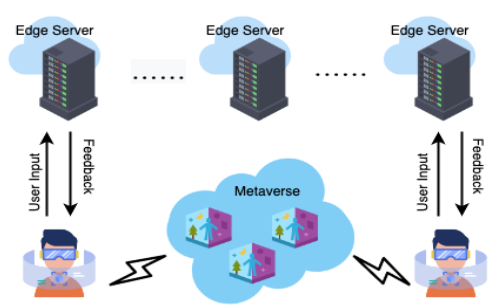
\includegraphics[width=0.85\textwidth]{images/existingArchitectres/mecBaseArch.png}
    \caption{Architektura Metaverse opartego na Mobile Edge Computing}
    \label{mecBaseArch}
\end{figure}

\newpage
Architektura oparta na przetwarzaniu we mgle proponuje wielopoziomowe podejście, w którym różne zadania obliczeniowe są dystrybuowane w warstwach mgły, krawędzi i chmury w celu optymalizacji wydajności i zmniejszenia wąskich gardeł obliczeniowych.

Artykuł podkreśla znaczenie \akronim{MEC} w infrastrukturze Metaverse poprzez rozwiązywanie krytycznych kwestii, takich jak opóźnienia, wydajność przepustowości i zarządzanie zasobami obliczeniowymi. Przybliżając moc obliczeniową do użytkowników końcowych i wykorzystując zaawansowaną infrastrukturę sieciową, taką jak \akronim{5G}, paradygmat \akronim{MEC} jest niezbędny do implementacji płynnego i wciągającego świata Metaverse.

\section{Dynamic Resource Allocation for Metaverse Applications with Deep Reinforcement Learning}

Artykuł "Dynamic Resource Allocation for Metaverse Applications with Deep Reinforcement Learning" autorstwa Nam H. Chu,
Eryk Dutkiewicz, Diep N. Nguyen, Dinh Thai Hoang, Khoa T. Phan, Dusit Niyato i Tao Shu koncentruje się na infrastrukturze i aspektach technicznych wymaganych do efektywnego zarządzania ogromnym zapotrzebowaniem na zasoby aplikacji Metaverse.

\subsection{Wyzwania związane z zarządzaniem zasobami}

Autorzy w artykule wskazują następujące wyzwania związane z zarządzaniem zasobami w środowisku Metaverse:

\begin{itemize}
    \item Aplikacje Metaverse wymagają dużych zasobów obliczeniowych, pamięci masowej i sieci, które przekraczają możliwości istniejących systemów.
    \item Dynamiczny i niepewny charakter żądań użytkowników i cykli życia aplikacji wymaga zaawansowanych strategii zarządzania zasobami.
\end{itemize}

\subsection{Proponowane rozwiązania}

Autorzy proponują następujące rozwiązania:
\begin{itemize}
    \item MetaInstancje i MetaSlices --- Aplikacje są podzielone na MetaInstancje, w których funkcje mogą być współdzielone między aplikacjami w celu zwiększenia efektywności wykorzystania zasobów.
    \item Architektura wielowarstwowa --- Framework wykorzystuje wielowarstwową architekturę chmury obliczeniowej do efektywnej dystrybucji zasobów z chmury do brzegu sieci, zmniejszając opóźnienia i przeciążenia.
\end{itemize}

\subsection{Wielowarstwowa architektura obliczeniowa}

Warstwowa dystrybucja zasobów zaprezentowana na rys.\ref{metaslicingMultiTierArch} zapewnia, że zasoby są dystrybuowane na wielu poziomach, od użytkowników końcowych po serwery w chmurze, aby zrównoważyć obciążenie i zoptymalizować wydajność.

\begin{figure}[!htbp]
    \centering
    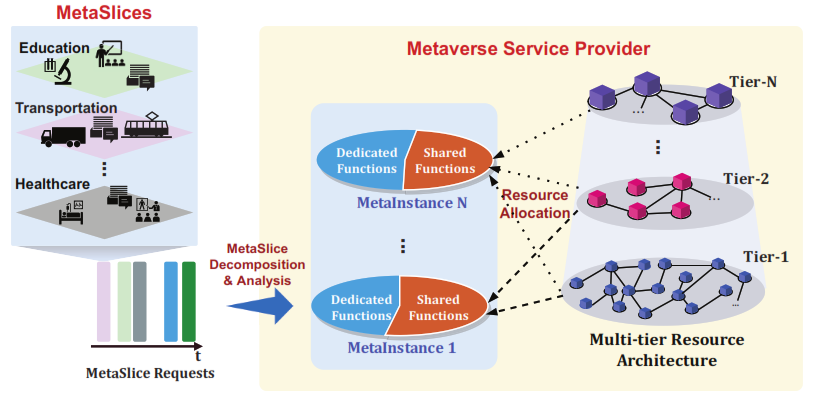
\includegraphics[width=\textwidth]{images/existingArchitectres/dynamicResourcemetaslicingMultiTierArch.png}
    \caption{Warstwowa dystrybucja zasobów}
    \label{metaslicingMultiTierArch}
\end{figure}

Dekompozycja aplikacji powoduje że aplikacje są dzielone na mniejsze funkcje, z których każda jest wykonywana na różnych poziomach w oparciu o ich wymagania dotyczące zasobów i dostępne możliwości.

\subsection{Dynamiczna alokacja zasobów}

Semi-Markov Decision Process \akronim{sMDP} --- Proces ten oddaje dynamiczne i niepewne cechy żądań zasobów i odejść aplikacji w czasie rzeczywistym.
Deep Reinforcement Learning \akronim{DRL} --- Opracowano inteligentny algorytm, który uczy się optymalnej polityki alokacji zasobów, maksymalizując wykorzystanie zasobów i przychody dostawcy przy jednoczesnym zachowaniu jakości usług.

\subsection{Inteligentny algorytm}

Deep Q-learning Techniques --- Algorytm wykorzystuje takie techniki, jak mechanizm odtwarzania bufora, architektura pojedynkowej sieci neuronowej i podwójne uczenie Q, aby ustabilizować proces uczenia się i uniknąć kwestii przeszacowania.

Optymalne uczenie się polityki --- System uczy się podejmować optymalne decyzje w zakresie kontroli dostępu w czasie rzeczywistym, dostosowując się do zmieniających się warunków i wymagań.\\

Artykuł przedstawia zaawansowany framework do dynamicznego zarządzania i alokacji zasobów w Metaverse przy użyciu kombinacji wielowarstwowego przetwarzania w chmurze i zaawansowanych technik głębokiego uczenia ze wzmocnieniem. Dzięki dekompozycji aplikacji na MetaSlices i MetaInstances oraz zastosowaniu procesu decyzyjnego semi-Markova, framework skutecznie radzi sobie z ogromnym i dynamicznym zapotrzebowaniem na zasoby aplikacji Metaverse.

\section{Unlocking Metaverse-as-a-Service}

Artykuł "Unlocking Metaverse-as-a-Service" autorstwa Vesal Ahsani, Ali Rahimi, 
Mehdi Letafati, Babak Hossein Khalaj, omawia niezbędną infrastrukturę techniczną i wyzwania związane z wdrażaniem platform Metaverse-as-a-Service \akronim{MaaS}.

\subsection{Główne filary MaaS}

Autorzy wskazują trzy główne filary:
\begin{itemize}
    \item Prywatność i bezpieczeństwo --- Zapewnienie bezpiecznych i prywatnych interakcji w Metaverse jest najważniejsze. Artykuł kładzie nacisk na mechanizmy prywatyzacji wrażliwych atrybutów danych i zabezpieczania rozproszonych algorytmów uczenia maszynowego.
    \item Przetwarzanie brzegowe --- wzmacnia Metaverse poprzez zmniejszenie opóźnień i przeciążenia sieci. Obejmuje przetwarzanie i przechowywanie danych blisko użytkowników końcowych, zwiększając wydajność i skalowalność aplikacji Metavers
    \item Technologia Blockchain --- Blockchain zapewnia przejrzystość, integralność danych i bezpieczne transakcje w ramach Metaverse. Obsługuje zdecentralizowane aplikacje i inteligentne kontrakty, niezbędne dla ekonomicznej i operacyjnej integralności Metaverse.
\end{itemize}

\subsection{Przetwarzanie brzegowe w Maas}

Struktura \akronim{MaaS} opiera się w dużej mierze na przetwarzaniu brzegowym, w którym przetwarzanie i przechowywanie danych odbywa się blisko użytkowników, zmniejszając opóźnienia i poprawiając wrażenia użytkownika. Serwery brzegowe mają kluczowe znaczenie dla obsługi lokalnego przetwarzania danych, pamięci masowej i funkcji sieciowych. Odciążają intensywne zadania z centralnych serwerów w chmurze, optymalizując ruch sieciowy i zwiększając możliwości przetwarzania danych w czasie rzeczywistym.

\subsection{Infrastruktura sieciowa}

Sieci 5G/6G --- Szybkie sieci bezprzewodowe o niskich opóźnieniach są niezbędne do obsługi wymagań Metaverse w czasie rzeczywistym. Sieci te ułatwiają płynny transfer danych między urządzeniami brzegowymi a serwerami. 

Bramy internetowe --- Łączą one systemy brzegowe z szerszą infrastrukturą sieciową i chmurową, zapewniając wydajny przepływ danych.

\subsection{Zarządzanie danymi i bezpieczeństwo}

Kontrola danych --- Przetwarzanie brzegowe zwiększa kontrolę nad danymi, utrzymując je blisko źródła, zapewniając lepsze zarządzanie prywatnością i bezpieczeństwem. Ma to kluczowe znaczenie dla obsługi danych wrażliwych, takich jak dane biometryczne i informacje zdrowotne.
Bezpieczna wymiana danych: Technologia Blockchain zapewnia, że dane udostępniane w ramach Metaverse są bezpieczne i niezmienne. Technologia ta wspiera bezpieczne transakcje i interakcje między użytkownikami i aplikacjami.

\subsection{Optymalizacja wydajności}

Przetwarzając dane na brzegu sieci, platforma znacząco redukuje opóźnienia, co ma kluczowe znaczenie dla aplikacji działających w czasie rzeczywistym, takich jak AR/VR i interaktywne gry.
Przetwarzanie brzegowe optymalizuje przepustowość sieci poprzez lokalne przetwarzanie danych, zmniejszając potrzebę przesyłania dużych ilości danych do centralnych serwerów.

Artykuł przedstawia infrastrukturę techniczną wymaganą do obsługi platform Metaverse-as-a-Service, koncentrując się na prywatności i bezpieczeństwie, przetwarzaniu brzegowym i technologii blockchain. Przetwarzanie brzegowe odgrywa kluczową rolę w zmniejszaniu opóźnień i optymalizacji wydajności sieci, podczas gdy blockchain zapewnia integralność danych i bezpieczne transakcje. Integracja tych technologii tworzy solidne, skalowalne i bezpieczne ramy dla Metaverse, zdolne do obsługi rozległych i dynamicznych wymagań dotyczących zasobów w immersyjnych środowiskach wirtualnych.
